\documentclass[a4paper,12pt]{article} % добавить leqno в [] для нумерации слева
\usepackage[a4paper,top=1.3cm,bottom=2cm,left=1.5cm,right=1.5cm,marginparwidth=0.75cm]{geometry}
%%% Работа с русским языком
\usepackage{cmap}					% поиск в PDF
\usepackage{mathtext} 				% русские буквы в фомулах
\usepackage[T2A]{fontenc}			% кодировка
\usepackage[utf8]{inputenc}			% кодировка исходного текста
\usepackage[english,russian]{babel}	% локализация и переносы

\usepackage{graphicx}

\usepackage{wrapfig}
\usepackage{tabularx}

\usepackage{subcaption,floatrow,graphicx,calc}
\usepackage{wrapfig}

% Создаёем новый разделитель
\DeclareFloatSeparators{mysep}{\hspace{1cm}}

% Ссылки?
\usepackage{hyperref}
\usepackage[rgb]{xcolor}
\hypersetup{				% Гиперссылки
    colorlinks=true,       	% false: ссылки в рамках
	urlcolor=blue          % на URL
}


\usepackage{hyperref}
\usepackage[rgb]{xcolor}
\hypersetup{
colorlinks=true,urlcolor=blue
}
\usepackage{multirow}
\usepackage{hhline}


%%% Дополнительная работа с математикой
\usepackage{amsmath,amsfonts,amssymb,amsthm,mathtools} % AMS
\usepackage{icomma} % "Умная" запятая: $0,2$ --- число, $0, 2$ --- перечисление

%% Номера формул
\mathtoolsset{showonlyrefs=true} % Показывать номера только у тех формул, на которые есть \eqref{} в тексте.

%% Шрифты
\usepackage{euscript}	 % Шрифт Евклид
\usepackage{mathrsfs} % Красивый матшрифт

%% Свои команды
\DeclareMathOperator{\sgn}{\mathop{sgn}}

%% Перенос знаков в формулах (по Львовскому)
\newcommand*{\hm}[1]{#1\nobreak\discretionary{}
{\hbox{$\mathsurround=0pt #1$}}{}}

\begin{document}

\newenvironment{lines}[1][\textwidth] % по умолчанию линейки на всю ширину текста
{
\newcolumntype{E}{>{}p{#1}<{\hrulefill}} % в конце нашего столбца будет приписываться \hrulefill
\begin{flushright} % автоматически вставим flushright
\begin{tabular}[h]{E} % и tabular нужного формата
}
{\end{tabular}\end{flushright}
}
	
	\begin{titlepage}
	\begin{center}
		{\large МОСКОВСКИЙ ФИЗИКО-ТЕХНИЧЕСКИЙ ИНСТИТУТ (НАЦИОНАЛЬНЫЙ ИССЛЕДОВАТЕЛЬСКИЙ УНИВЕРСИТЕТ)}
	\end{center}
	\begin{center}
		{\large Физтех-школа электроники, фотоники и молекулярной физики}
	\end{center}
	
	
	\vspace{4.5cm}
	{\huge
		\begin{center}
			{Лабораторная работа 5.4.1}\\
			Определение энергии $\alpha$-частиц\\по величине их пробега в воздухе
		\end{center}
	}
	\vspace{2cm}
	\begin{flushright}
		{\LARGE Салтыкова Дарья \\
			\vspace{0.5cm}
			Б04-105}
	\end{flushright}
	
	\vspace{0.5cm}
	
	\begin{lines}[.5
	\textwidth]
  {\LARGE Допуск} \rule{6.5cm}{0.25pt} \vspace{0.5cm}\\
 {\LARGE Выполнение} \rule{3cm}{0.25pt}\vspace{0.5cm} \\ {\LARGE Сдача} \rule{3cm}{0.25pt} \\ % \rule сделает линейку указанной длины и толщины
\end{lines}
	\vspace{6cm}
	\begin{center}
		Долгопрудный 2023
	\end{center}
\end{titlepage}

\section{Введение}

\noindent
\textbf{Цель работы:} измерить пробег $\alpha$-частиц в воздухе двумя способами: с помощью торцевого счетчика Гейгера и синтиляционного счетчика, -- по полученным данным определить энергию частиц.


\medskip

\section{Теоретические сведения}
	При $\alpha$-распаде исходное родительское ядро испускает ядро гелия и превращается в дочернее ядро, число протонов и число протонов уменьшается на две единицы. Функциональная свзяь между энергией $\alpha$-частицы $E$ и периодом полураспада радиоактивного ядра $T_{1/2}$ хорошо описывается формулой
	\begin{equation*}
		 \lg T_{1/2} = \frac{a}{\sqrt{E}} + b.
	\end{equation*}
	Экспоненциальный характер этого процесса возникает вследствие экспоненциального затухания волновой функции в области под барьером, где потенциальная энергия больше энергии частицы.
	
	\medskip

\noindent Для описания связи между энергией $\alpha$-частицы и ее пробегом пользуются эмпирическими соотношениями. В диапазоне энергий $\alpha$-частиц от 4 до 9 МэВ эта связь хорошо описывается выражением

	\begin{equation*}
		\label{eq:R(E)}
		\tag{$\star$}
		R = 0,32E^{3/2}
	\end{equation*}
	

\section{Экспериментальная установка}

	В данной работе пробег $\alpha$-частиц в воздухе определяется треями способами:
	\begin{enumerate}
		\item
			С помощью счетчика Гейгера -- рис.~\ref{pic1};
		\item
			C помощью сцинтилляционного счетчика -- рис.~\ref{pic2};
		\item
			C помощью ионизационной камеры -- рис.~\ref{pic3}.
	\end{enumerate} 
	
	\thisfloatsetup{floatrowsep=mysep}	
	\begin{figure}[h!]
		\ffigbox{
			\begin{subfloatrow}[3]
				\ffigbox[\FBwidth]{\caption{}}%
				{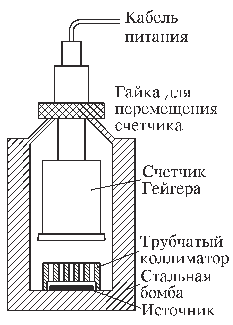
\includegraphics[scale=1]{ustanovka1.pdf}{\label{pic1}}}
				\ffigbox[\FBwidth]{\caption{}}%
				{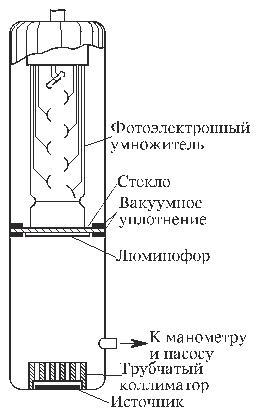
\includegraphics[scale=0.8]{ustanovka2.pdf}{\label{pic2}}}
				\ffigbox[\FBwidth]{\caption{}}%
				{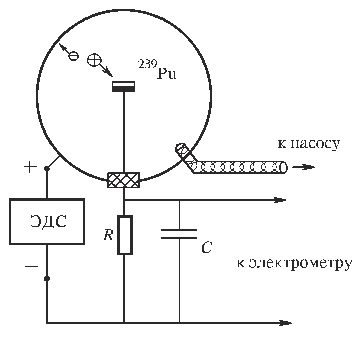
\includegraphics[scale=1]{ustanovka3.pdf}{\label{pic3}}}          
			\end{subfloatrow}
		}
		{\caption{Экспериментальные установки.}}
	\end{figure}
	
\noindent В качестве источника $\alpha$-частиц используется ${239}$Pu с периодом полураспада $T_{1/2} = 2,44 \cdot 10^4$ лет. Альфа-частицы, испускаемые ${239}$Pu состоят их трех моноэнергетических групп, различие между которыми лежит в пределах 50 кэВ. При той точности, которая достигается в наших опытах, их можно считать совпадающими по энергии, равной 5,15 МэВ.
	
\newpage

\section{Ход работы}

\subsection{I. Ионизационная камера}

\noindent 1. Найдем длину свободного пробега, используя ионизационную камеру. Измерим начальные параметры. Атмосферное давление по барометру: $P_A = 100,9 \text{ кПа} = 756,8 \text{ Торр}.$ Ток $8,93 \text{ пА}.$ Температура $T = 298 K.$

\medskip

\noindent 2. Откачаем воздух из камеры до давления порядка $\approx 10 \text{ Торр}.$

\medskip

\noindent 3. Построим график зависимости I(P). (Данные см. в Приложении).

\begin{figure}[h!]
    \centering
    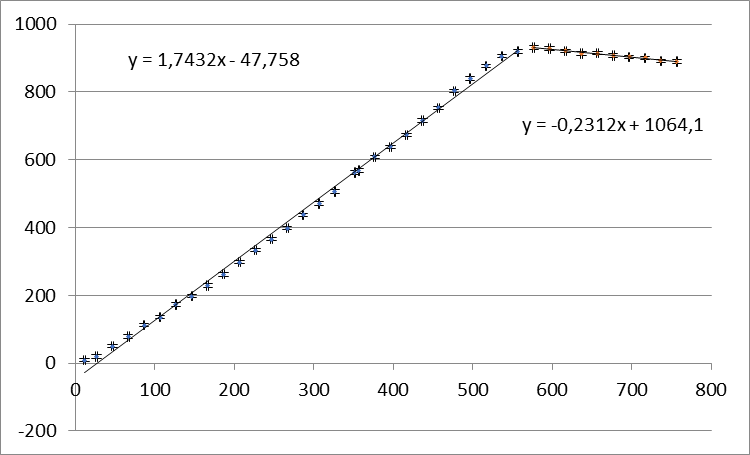
\includegraphics[scale=0.8]{1.png}
    \caption{I(P)}
    
\end{figure}

\noindent Определим по графику $P_{\text{экстр}} = (563 \pm 10)\text{ Торр}.$
\medskip

\noindent Тогда экстраполированный пробег и соответствующая энергия:
$$R_{\text{экстр}} = \frac{288}{T} \frac{P}{760} \frac{10 - 0,5}{2} = 4,57 \pm 0,08 \text{ см}$$

$$E(R_{\text{экстр}} = (5,89 \pm 0,07) \text{ МэВ}.$$

\subsection{II.Сцинтилляционный счетчик}

\noindent 1. Подадим напряжение на ФЭУ и измерим скорость счета при $P_A$.

\medskip

\noindent 2. Откачаем камеру. Снимем зависимость N(P) (данные см. в Приложении) и построим ее график.

\begin{figure}[h!]
    \centering
    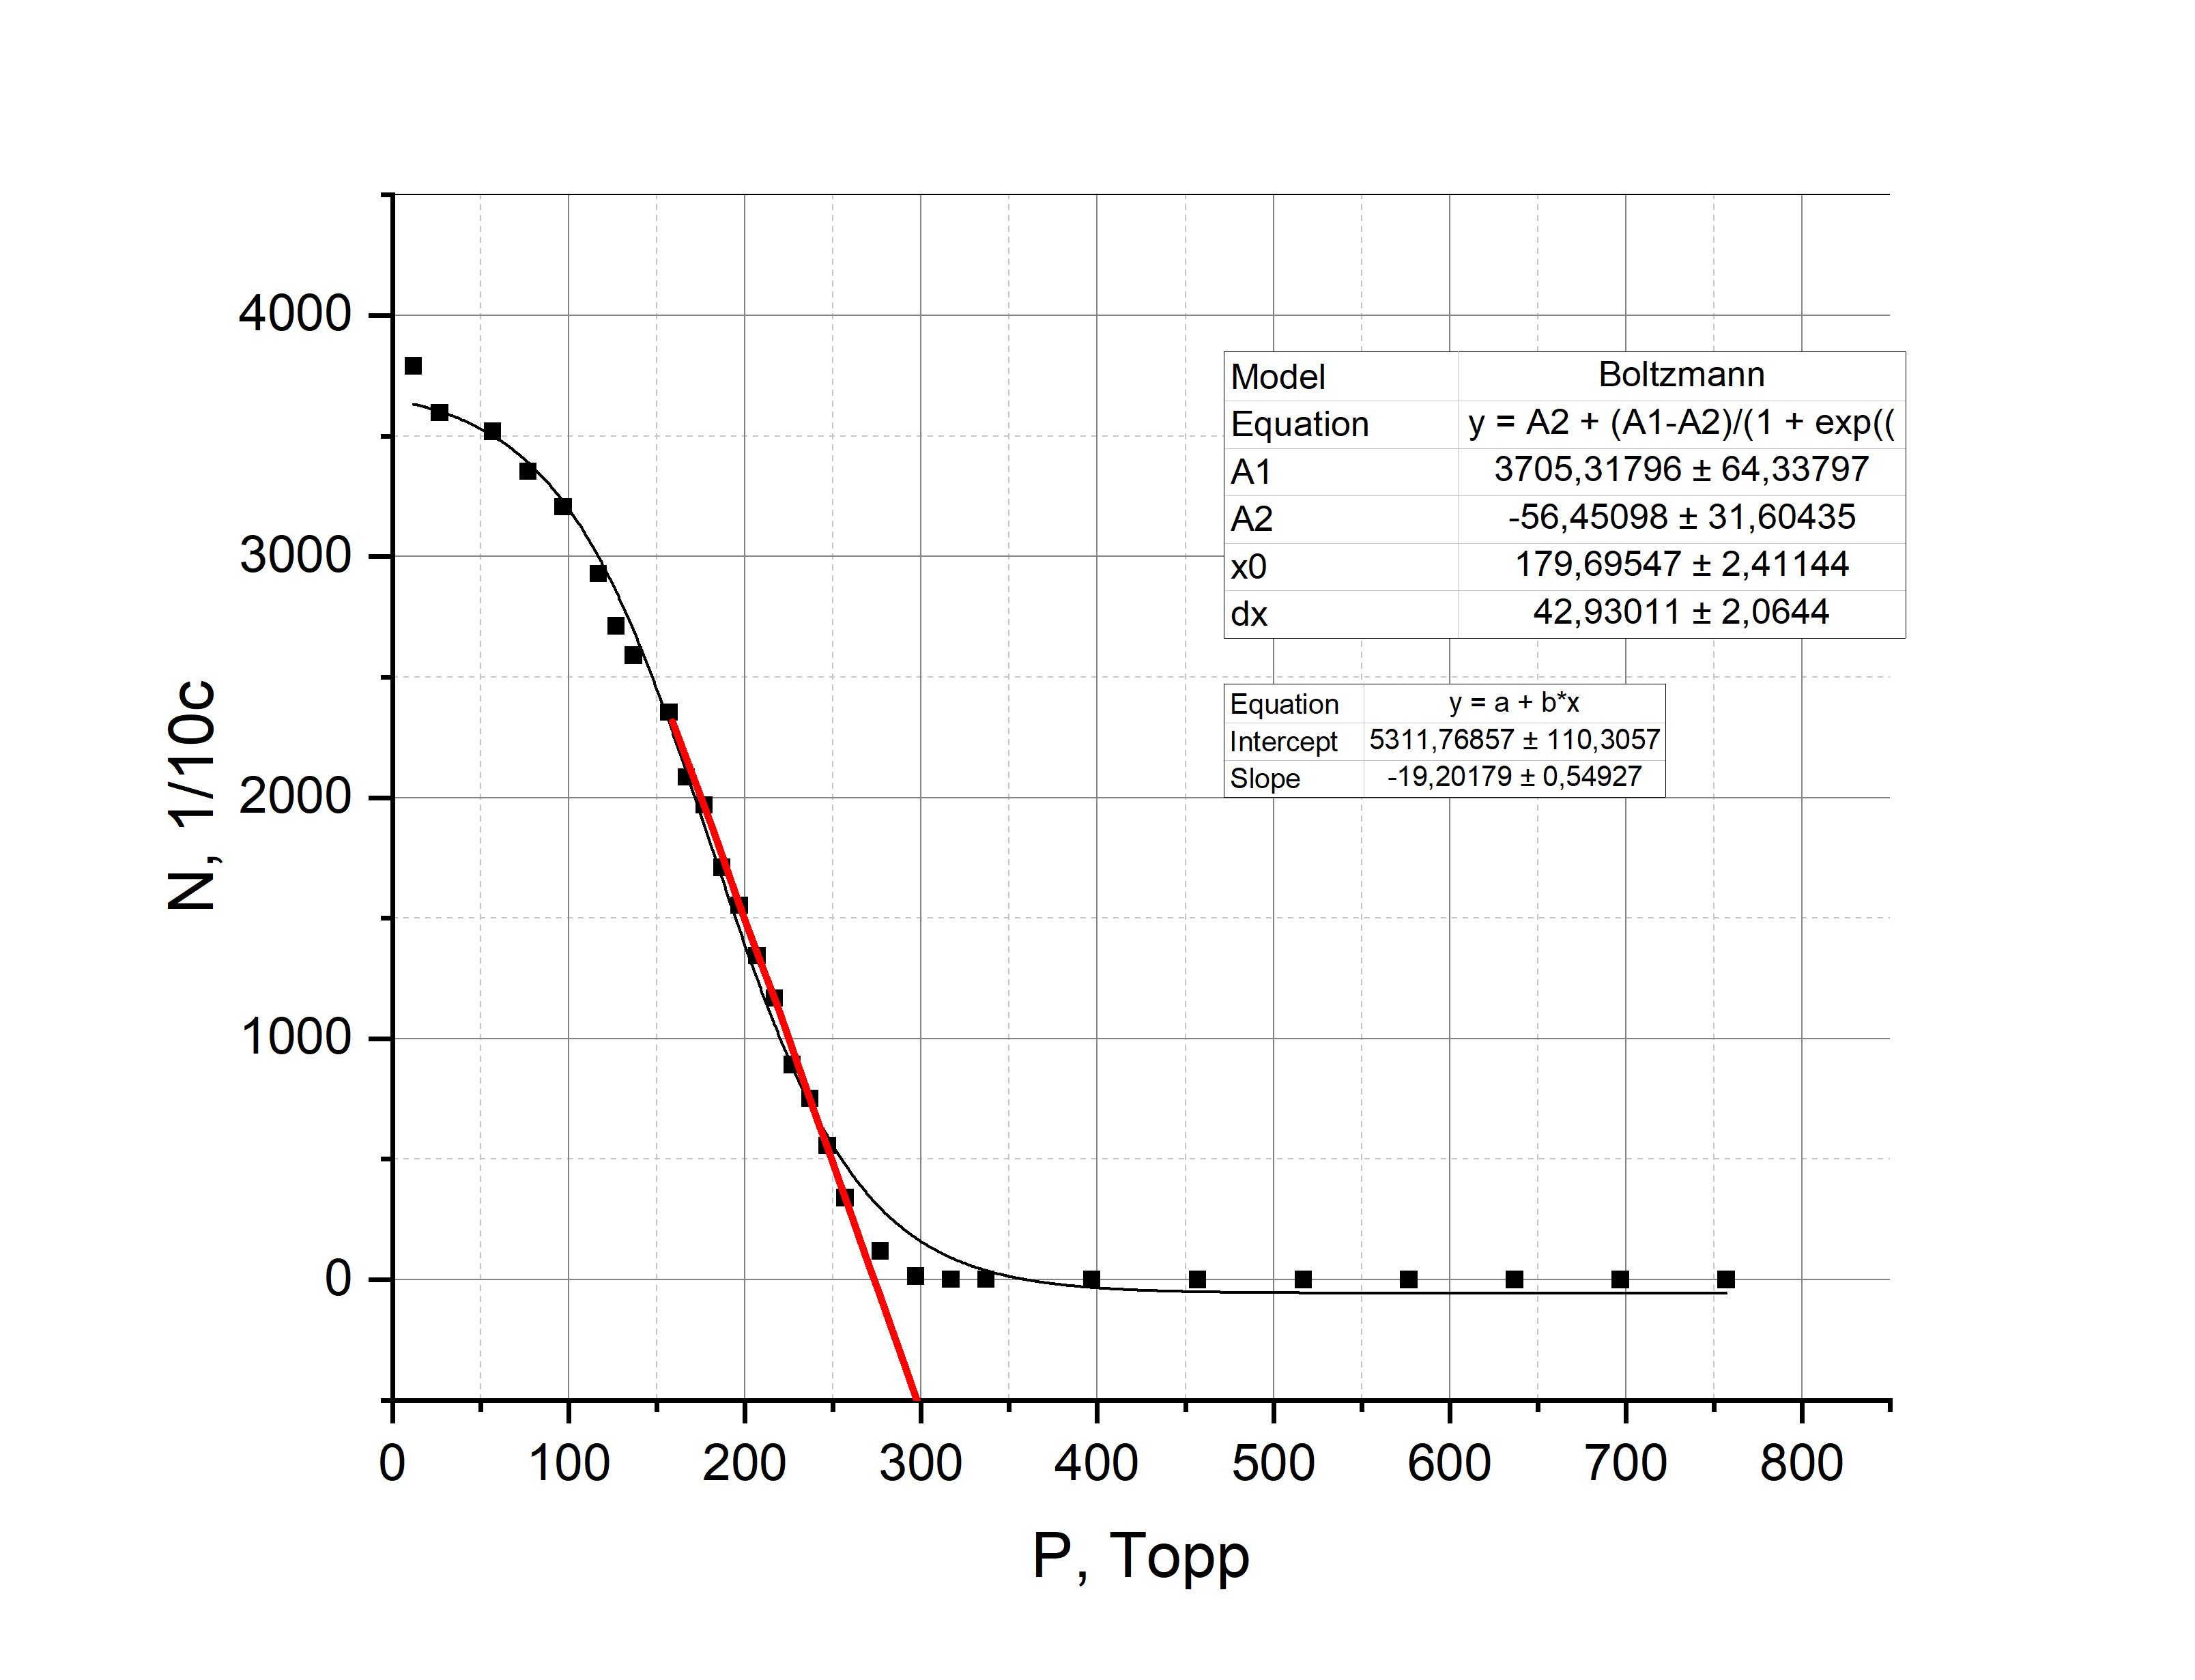
\includegraphics[scale=0.5]{2.png}
    \caption{$N(P)$}
    
\end{figure}

\noindent Кривую, приближающую экспериментальные точки, будем искать в виде
$$N(P) = A2 + \frac{A_1 - A_2}{1 + e^{\frac{P-P_0}{dP}}}.$$

\medskip

\noindent Параметры аппроксимации, определенные с помощью Origin: $A_1 = 3705 \pm 64, A_2 = -56 \pm 31, P_0 = 180 \pm 2, dP = 43 \pm 2.$

\medskip

\noindent 3. Найдем $P_{\text{ср}}$ и $P_{\text{экстр}}$, а по ним $R_{\text{ср}}$ и $R_{\text{экстр}}$.

\medskip 

$$N''(P_{\text{ср}}) = 0$$
$$P_{\text{ср}} = (180 \pm 4) \text{ Торр}, R_{\text{ср}} = \frac{288}{T} \cdot \frac{P}{760} \cdot 9 = 2,06 \pm 0,05 \text{ см}.$$

\noindent Построим касательную к кривой N(P) через точку $P_{\text{ср}}$ и продолжим ее до пересечения с осью P. Получим $P_{\text{экстр}} = (294 \pm 8) \text{ Торр}, R_{\text{экстр}} = 3,17 \pm 0,09 \text{ см}.$ 

\medskip

\noindent Тогда $E(R_{\text{ср}} = (3,46 \pm 0,06) \text{ МэВ}), E(R_{\text{экстр}}) = (4,61 \pm 0,09) \text{ МэВ}$.

\medskip

\noindent 4. Рассчитаем по полученным данным, бумажный листок какой толщины не пропустит $\alpha$-частицы от $^{239} Pu$. Если плотность бумаги 1,2 г/см^2, то $L \ge R/\rho = 32,4 мкм.$

\section{Вывод}

\noindent В данной работе была двумя способами измерена длина свободного пробега $\alpha$-частиц в воздухе: с помощью ионизационной камеры и сцинтилляционного счетчика. Получены следующие результаты:

$$R_{\text{ср}} = 2,06 \pm 0,05 \text{ см}, E(R_{\text{ср}} = (3,46 \pm 0,06) \text{ МэВ}),$$
$$R_{\text{экстр}} = 3,17 \pm 0,09 \text{ см}, E(R_{\text{экстр}}) = (4,61 \pm 0,09) \text{ МэВ}  \text{ -- для сцинтилляционного счетчика};$$

$$R_{\text{экстр}} =(4,57 \pm 0,08) \text{ см}, E(R_{\text{экстр}} = (5,89 \pm 0,07) \text{ МэВ}  \text { -- для ионизационной камеры}.$$

$$E_{\text{табл}} = 5,15 \text{ МэВ}.$$

\medskip

\noindent Несоответствие экспериментальных значений табличному может быть связано или с заметной угловой расходимостью пучков (брэгговский пик смещен и сильно размыт), или с тем, что пленка, покрывающая источники, замедляет движение альфа-частиц.

\medskip
 
\noindent Также было оценено, что бумажный листок толщиной более 32,4 мкм не пропустит $\alpha$-частицы от $^{239} Pu$.

\newpage

\section{Приложение}

\begin{table}[h!]
\begin{tabular}{|ll|l|l|}
\hline
\multicolumn{2}{|l|}{$\delta P,  \text{ Торр}$} & $I, \text{ пА}$ & $P, \text{ Торр}$ \\ \hline
\multicolumn{1}{|l|}{745}        & 0,11        & 9               & 11,8              \\ \hline
\multicolumn{1}{|l|}{730}        & 0,22        & 20              & 26,8              \\ \hline
\multicolumn{1}{|l|}{710}        & 0,52        & 50              & 46,8              \\ \hline
\multicolumn{1}{|l|}{690}        & 0,81        & 79              & 66,8              \\ \hline
\multicolumn{1}{|l|}{670}        & 1,14        & 112             & 86,8              \\ \hline
\multicolumn{1}{|l|}{650}        & 1,38        & 136             & 106,8             \\ \hline
\multicolumn{1}{|l|}{630}        & 1,75        & 173             & 126,8             \\ \hline
\multicolumn{1}{|l|}{610}        & 2           & 198             & 146,8             \\ \hline
\multicolumn{1}{|l|}{590}        & 2,31        & 229             & 166,8             \\ \hline
\multicolumn{1}{|l|}{570}        & 2,64        & 262             & 186,8             \\ \hline
\multicolumn{1}{|l|}{550}        & 3           & 298             & 206,8             \\ \hline
\multicolumn{1}{|l|}{530}        & 3,35        & 333             & 226,8             \\ \hline
\multicolumn{1}{|l|}{510}        & 3,68        & 366             & 246,8             \\ \hline
\multicolumn{1}{|l|}{490}        & 4           & 398             & 266,8             \\ \hline
\multicolumn{1}{|l|}{470}        & 4,39        & 437             & 286,8             \\ \hline
\multicolumn{1}{|l|}{450}        & 4,73        & 471             & 306,8             \\ \hline
\multicolumn{1}{|l|}{430}        & 5,08        & 506             & 326,8             \\ \hline
\multicolumn{1}{|l|}{405}        & 5,64        & 562             & 351,8             \\ \hline
\multicolumn{1}{|l|}{400}        & 5,7         & 568             & 356,8             \\ \hline
\multicolumn{1}{|l|}{380}        & 6,1         & 608             & 376,8             \\ \hline
\multicolumn{1}{|l|}{360}        & 6,4         & 638             & 396,8             \\ \hline
\multicolumn{1}{|l|}{340}        & 6,75        & 673             & 416,8             \\ \hline
\multicolumn{1}{|l|}{320}        & 7,18        & 716             & 436,8             \\ \hline
\multicolumn{1}{|l|}{300}        & 7,55        & 753             & 456,8             \\ \hline
\multicolumn{1}{|l|}{280}        & 8,05        & 803             & 476,8             \\ \hline
\multicolumn{1}{|l|}{260}        & 8,42        & 840             & 496,8             \\ \hline
\multicolumn{1}{|l|}{240}        & 8,79        & 877             & 516,8             \\ \hline
\multicolumn{1}{|l|}{220}        & 9,07        & 905             & 536,8             \\ \hline
\multicolumn{1}{|l|}{200}        & 9,21        & 919             & 556,8             \\ \hline
\multicolumn{1}{|l|}{180}        & 9,33        & 931             & 576,8             \\ \hline
\multicolumn{1}{|l|}{160}        & 9,3         & 928             & 596,8             \\ \hline
\multicolumn{1}{|l|}{140}        & 9,23        & 921             & 616,8             \\ \hline
\multicolumn{1}{|l|}{120}        & 9,15        & 913             & 636,8             \\ \hline
\multicolumn{1}{|l|}{100}        & 9,16        & 914             & 656,8             \\ \hline
\multicolumn{1}{|l|}{80}         & 9,09        & 907             & 676,8             \\ \hline
\multicolumn{1}{|l|}{60}         & 9,05        & 903             & 696,8             \\ \hline
\multicolumn{1}{|l|}{40}         & 9,02        & 900             & 716,8             \\ \hline
\multicolumn{1}{|l|}{20}         & 8,94        & 892             & 736,8             \\ \hline
\multicolumn{1}{|l|}{0}          & 8,92        & 890             & 756,8             \\ \hline
\end{tabular}
\end{table}

\newpage

\begin{table}[h!]
\begin{tabular}{|l|l|l|}
\hline
$\delta P, \text{ Торр}$ & $t, \text{с}$ & $N$  \\ \hline
745                      & 10            & 3791 \\ \hline
730                      & 10            & 3597 \\ \hline
700                      & 10            & 3519 \\ \hline
680                      & 10            & 3354 \\ \hline
660                      & 10            & 3206 \\ \hline
640                      & 10            & 2929 \\ \hline
620                      & 10            & 2591 \\ \hline
600                      & 10            & 2354 \\ \hline
580                      & 10            & 1969 \\ \hline
560                      & 10            & 1554 \\ \hline
540                      & 10            & 1168 \\ \hline
520                      & 10            & 753  \\ \hline
500                      & 10            & 341  \\ \hline
480                      & 10            & 120  \\ \hline
460                      & 10            & 15   \\ \hline
440                      & 10            & 2    \\ \hline
420                      & 100           & 20   \\ \hline
360                      & 100           & 13   \\ \hline
300                      & 100           & 7    \\ \hline
240                      & 100           & 6    \\ \hline
180                      & 100           & 6    \\ \hline
120                      & 100           & 6    \\ \hline
60                       & 100           & 6    \\ \hline
0                        & 100           & 6    \\ \hline
630                      & 10            & 2712 \\ \hline
590                      & 10            & 2085 \\ \hline
570                      & 10            & 1711 \\ \hline
550                      & 10            & 1344 \\ \hline
530                      & 10            & 892  \\ \hline
510                      & 10            & 557  \\ \hline
\end{tabular}
\end{table}

\end{document}